\section{Construction}
\label{sec.construction}

A client receives a chain and keeps a prefix of it. This section says which
prefix.

It cannot keep all of it. The chain it was handed may fork off every chain the
honest validators hold, and the blocks after that fork are on no honest chain.
It cannot find the fork either. It has one chain and nothing to compare it
against. What it can do is put a bound on how deep the fork goes, using only the
height of the chain and the round.

Let the client receive at round $r$ a chain $\ch$ of height $\hgt$. Let $\rst$ be the
round in which the fork point was mined, and let $d$ be the number of blocks
that come after it. Two facts bound $d$. The first is that no chain is taller
than about $(1+\advr)f\rst$ at round $\rst$, so the fork point is no higher than
that, and
\begin{equation}\label{eq.early}
    \hgt \lesssim (1+\advr)f\rst + d .
\end{equation}
The second is that only adversarial blocks extend a fork, and the adversary
finds about $\advr f$ blocks per round, so
\begin{equation}\label{eq.deep}
    d \lesssim \advr f(r-\rst) .
\end{equation}
Both inequalities constrain $\rst$, and they constrain it from opposite sides.
\Cref{eq.early} rearranges to $\rst\gtrsim(\hgt-d)/((1+\advr)f)$: the fork point
needed that long to reach its height. \Cref{eq.deep} rearranges to
$\rst\lesssim r-d/(\advr f)$: the adversary needed that long to mine the $d$
blocks above it. A round satisfying both exists only while $d$ is small enough,
and eliminating $\rst$ between them gives
\begin{equation}\label{eq.idealdepth}
    d \lesssim \advr\left((1+\advr)fr - \hgt\right) .
\end{equation}
The client prunes that many blocks. We write $\prn(r,\hgt)$ for the number it
prunes and $\pref(r,\hgt)=\hgt-\prn(r,\hgt)$ for the height of what is left, the
confirmed height. Both read only the round and the height. The three bounds above are approximate. The rest of this section
replaces them by rates that hold in every typical execution, and
\Cref{sec.analysis} proves the result sound.

\paragraph{Normalised form}

It helps to measure the chain against what an honest chain would be. Write
$\rate=\hgt/(fr)$ for its height in units of $fr$. Dividing
\Cref{eq.idealdepth} by $fr$ gives
\begin{equation}\label{eq.normal}
    \frac{d}{fr} \lesssim \advr\left(1+\advr-\rate\right),
    \qquad\text{so}\qquad
    \frac{\hgt-d}{fr} \gtrsim (1+\advr)\left(\rate-\advr\right) .
\end{equation}
One number now carries the whole rule, and three of its values matter. At
$\rate=1+\advr$ the chain is as tall as any chain can be, and the client prunes
nothing. At $\rate=1$ it is as tall as an honest chain, and the client prunes an
$\advr^2$ fraction of it. At $\rate=\advr$ it is no taller than what the
adversary could have built alone, and nothing is kept. \Cref{fig.confirmed}
draws this, and \Cref{cor.limit} proves it.

\begin{figure}[t]
\centering
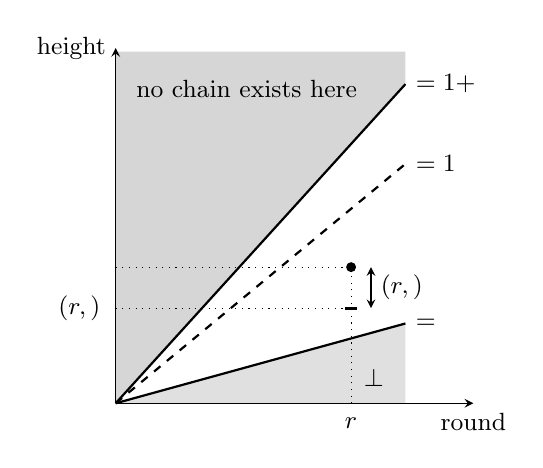
\begin{tikzpicture}[x=1.15cm,y=0.95cm,>=stealth,font=\small]
  % rho = 1/3: the three rays have slopes 4/3, 1 and 1/3.
  \def\xe{3.2}
  \def\yh{4.2667}   % top ray at \xe
  \def\ym{3.2}      % middle ray at \xe
  \def\yl{1.0667}   % bottom ray at \xe

  % regions
  \fill[black!12] (0,0) -- (\xe,\yl) -- (\xe,0) -- cycle;
  \fill[black!16] (0,0) -- (\xe,\yh) -- (\xe,4.7) -- (0,4.7) -- cycle;

  % axes
  \draw[->] (0,0) -- (3.95,0) node[below] {round};
  \draw[->] (0,0) -- (0,4.75) node[left] {height};

  % rays
  \draw[thick]        (0,0) -- (\xe,\yh) node[right] {$\rate=1+\advr$};
  \draw[thick,dashed] (0,0) -- (\xe,\ym) node[right] {$\rate=1$};
  \draw[thick]        (0,0) -- (\xe,\yl) node[right] {$\rate=\advr$};

  % the received chain at round r, of height alpha, and its confirmed prefix
  \def\xr{2.6}
  \def\ya{1.82}
  \def\yz{1.2711}
  \draw[dotted] (\xr,0) -- (\xr,\ya);
  \draw[dotted] (0,\ya) -- (\xr,\ya);
  \draw[dotted] (0,\yz) -- (\xr,\yz);
  \fill (\xr,\ya) circle (1.8pt);
  \draw[very thick] (\xr-0.07,\yz) -- (\xr+0.07,\yz);
  \draw[<->] (\xr+0.22,\yz) -- (\xr+0.22,\ya) node[midway,right] {$\prn(r,\hgt)$};

  \node[anchor=east] at (-0.06,\ya) {$\hgt$};
  \node[anchor=east] at (-0.06,\yz) {$\pref(r,\hgt)$};
  \node[anchor=north] at (\xr,-0.06) {$r$};

  \node[anchor=north west] at (0.12,4.45) {no chain exists here};
  \node at (2.85,0.34) {$\bot$};
\end{tikzpicture}
\caption{The confirmed height, drawn for $\advr=\frac{1}{3}$. A chain $\ch$ received
at round $r$ is a point at height $\hgt$. No chain reaches above the ray
$\rate=1+\advr$, and a chain adopted by an honest validator reaches at least
the ray $\rate=1$. The confirmed height $\pref(r,\hgt)$ interpolates linearly
between the two outer rays, equal to $\hgt$ on the upper one and to zero on the
lower one. The client prunes the difference $\prn(r,\hgt)$, and it outputs $\bot$
when the point falls below the lower ray.}\label{fig.confirmed}
\end{figure}


\paragraph{Pruning depth}

The exact rule replaces the approximate rates of \Cref{eq.early,eq.deep} by
bounds that hold in every typical execution. We use three constants. The first
is
\[
    \maxr = 1 + \advr + 2\epsilon + \frac{\advr f}{1-f} ,
\]
and $\maxr f$ is an upper bound on the growth rate of every chain, from
\Cref{lem.length}. It takes the place of $(1+\advr)f$ in \Cref{eq.early}. The
second is
\[
    \advrone = \frac{\advr}{1-f} + \frac{f_2}{f} + 2\epsilon ,
\]
the rate per round at which the adversary lengthens a fork, from
\Cref{eq.upper}. It takes the place of $\advr f$ in \Cref{eq.deep}. Neither
constant is far from $\advr$. Each exceeds it only by the collision rate $f_2/f$
and by multiples of $\epsilon$, and both tend to $\advr$ as $f$ and $\epsilon$
tend to $0$, while $\maxr$ tends to $1+\advr=n/(n-t)$. The third constant is
$k_0=2(\lambda+2)f$, which is the scale of the common prefix parameter
of~\cite{gkl24}. Since $\lambda\ge2/f$ we have $2\lambda f\le k_0\le4\lambda f$.
From \Cref{lem.fsq}, $f_2/f<f/(2(1-f)^2)$, and $f<1/3$ by
\Cref{asm.majority}, so $f_2/f<1$ and the pruning depth
\begin{equation}\label{eq.depth}
    \prn(r,\hgt)
    = \max\left\{k_0,\
    \frac{\advrone\left[\maxr f(r+\lambda)-\hgt+1\right]+\maxr(2f+1)}{1-f_2/f}\right\}
\end{equation}
is well defined. The confirmed height $\pref(r,\hgt)=\hgt-\prn(r,\hgt)$ then
reads, using $\maxr-\advrone=1-f_2/f$,
\begin{equation}\label{eq.pref}
    \pref(r,\hgt) = \min\Big\{\hgt-k_0,\
    \frac{\maxr}{1-f_2/f}\big(\hgt-h_0(r)\big)\Big\},
    \qquad h_0(r)=\advrone f(r+\lambda)+2f+1 .
\end{equation}
This is the same rule seen from below. The height $h_0(r)$ is about the number
of blocks the adversary alone can have mined by round $r$, and nothing below
it is confirmed. Whatever sits above it is confirmed, scaled by
$\frac{\maxr}{1-f_2/f}$, which tends to $1+\advr$.

\begin{definition}[Pruning client]\label{def.client}
    The pruning client is the following.
    \begin{enumerate}
        \item The client asks for a chain and waits until it receives one. Let
            $\ch$ be the chain received, let $\hgt$ be its height, and let $r$
            be the round of receipt.
        \item The client computes $\prn(r,\hgt)$ by \Cref{eq.depth}.
        \item If $\prune{\ch}{\prn(r,\hgt)}$ has more than one block, the client
            outputs it. Otherwise it outputs $\bot$.
    \end{enumerate}
\end{definition}

\begin{algorithm}
\caption{The client. It outputs $\ch_{\mathrm{out}}$ at every round.}\label{alg.client}
\begin{algorithmic}[1]
\State $\ch_{\mathrm{out}} \gets \bot$ \label{line.init}
\For{every valid chain $\ch$ received, at the round $r$ of its receipt}
    \State $k \gets \prn(r,\len{\ch}-1)$ \Comment{\Cref{eq.depth}} \label{line.depth}
    \State $\ch \gets \prune{\ch}{k}$ \label{line.prune}
    \If{$\len{\ch} > 1$ \textbf{and} ($\ch_{\mathrm{out}} = \bot$ \textbf{or} $\len{\ch} > \len{\ch_{\mathrm{out}}}$)} \label{line.compare}
        \State $\ch_{\mathrm{out}} \gets \ch$ \label{line.keep}
    \EndIf
\EndFor
\end{algorithmic}
\end{algorithm}


The rule reads two things: the round the chain arrived and its height. It does
not read the blocks of the chain, and it does not read the length of any chain
a validator holds. It does not need a
delay bound. It never asks whether whoever answered is honest.

\paragraph{Repeated confirmation}

A client that stays online is handed more than one chain. It runs
\Cref{def.client} on each and keeps whichever output is longest.

\begin{definition}[Monotone client]\label{def.monotone}
    The monotone client runs \Cref{def.client} on every chain it receives and
    outputs the longest chain that any of these runs has returned, or $\bot$ if
    every run returned $\bot$.
\end{definition}

This is well defined. \Cref{cor.consistency} shows that the outputs of
\Cref{def.client} are nested, so one of them is longest, and a client that keeps
it never has to take anything back.

Four results follow. \Cref{thm.safety} shows the output is a prefix of every
chain an honest validator adopts, at the round of receipt and at every round
after it. \Cref{cor.consistency} shows any two clients output prefixes of one
another. \Cref{thm.liveness} says how far behind the honest chain the output
sits. \Cref{cor.tight} shows no smaller pruning depth is sound.
